\documentclass[14pt]{extarticle}
\usepackage[english,ukrainian]{babel}
\usepackage[utf8]{inputenc}
\usepackage{amsmath,amssymb}
\usepackage{parskip}
\usepackage{graphicx}
\usepackage{xcolor}
\usepackage{tcolorbox}
\tcbuselibrary{skins}
\usepackage[framemethod=tikz]{mdframed}
\usepackage{chngcntr}
\usepackage{enumitem}
\usepackage{hyperref}
\usepackage{float}
\usepackage{subfig}
\usepackage{chngcntr}
\usepackage{esint}
\usepackage{subfig}
\usepackage[top=2.5cm, left=3cm, right=3cm, bottom=4.0cm]{geometry}
\usepackage[table]{xcolor}
\usepackage{algorithm}
\usepackage{algpseudocode}
\usepackage{listings}
\tcbuselibrary{theorems}

\newtcbtheorem[number within=section]{def}{Визначення}%
{colback=blue!5,colframe=blue!35!black,fonttitle=\bfseries}{th}

\title{Контрольна робота \#2 з курсу ``Диференціальні рівняння''}
\author{Студента 3 курсу групи МП-31 Захарова Дмитра}
\date{\today}

\begin{document}

\maketitle

\begin{center}
    \textbf{Варіант 5}
\end{center}

\section*{Завдання 1.} 

\textbf{Умова.} Дослідити на стійкість розв'язок задачі Коші за визначенням:
\[
\begin{cases}
    \dot{x} = x(x^2-1) \\
    x(0) = 1
\end{cases}
\]

\textbf{Розв'язок.} Знайдемо спочатку розв'язок у явному вигляді:
\[
\frac{dx}{x(x-1)(x+1)} = dt
\]
Помітимо, що
\[
\frac{1}{x(x-1)(x+1)} = -\frac{1}{x} + \frac{1}{2(x-1)} + \frac{1}{2(x+1)}
\]
Тому після інтегрування маємо
\[
-\ln x + \frac{1}{2}\ln (x-1) + \frac{1}{2}\ln (x+1) = t + C
\]
Або
\[
\boxed{x(t) = \pm\frac{1}{\sqrt{1+Ae^{2t}}}}
\]

Для нашої задачі Коші $x(0)=1$, маємо $x \equiv 1$, оскільки у нас вийде $A=0$. Далі скористаємося означенням стійкості за Ляпуновим. 

\begin{def*}{Стійкість за Ляпуновим}
Нехай маємо систему 
\[
\dot{\mathbf{x}}=f(\mathbf{x}),\;\mathbf{x}(t_0)=\mathbf{x}_0
\]
Розв'язок $\boldsymbol{\varphi}(t)$ є стійким за Ляпуновим при $t \to \infty$, якщо
\begin{gather*}
\forall \epsilon > 0 \; \exists \delta(\epsilon) > 0 \; \forall \mathbf{x}(t): \text{розв'язок рівняння} \\ \|\mathbf{x}(t_0)-\boldsymbol{\varphi}(t_0)\| < \delta(\epsilon) \implies \|\mathbf{x}(t)-\boldsymbol{\varphi}(t)\| < \epsilon \; \forall t \geq t_0
\end{gather*}
\end{def*}

Доведемо, що наш розв'язок не є стабільним. Будуємо протилежне твердження:
\[
\exists \epsilon > 0 \; \forall \delta > 0 \; \exists \mathbf{x}(t): \|\mathbf{x}(t_0)-\boldsymbol{\varphi}(t_0)\| < \delta \wedge \exists t_1 \geq t_0: \|\boldsymbol{x}(t_1) - \boldsymbol{\varphi}(t_1)\| \geq \epsilon
\]
Отже, покладемо $\epsilon = 0.01$ для конкретності. Тоді для нашого випадку:
\[
\forall \delta > 0 \; \exists A_{\delta} \in \mathbb{R}: \left|\frac{1}{\sqrt{1+A_{\delta}}}-1\right| < \delta \wedge \exists \tau \geq 0: \left|\frac{1}{\sqrt{1+A_{\delta}e^{2\tau}}}-1\right| \geq 0.01
\]
Візьмемо $A_{\delta}$, що буде задовольняти першій умові (оскільки функція $f(A_{\delta})=\left|\frac{1}{\sqrt{1+A_{\delta}}}-1\right|$ приймає усі значення від $0$ до $+\infty$). Далі вже в незалежності від знаку або значення $A_{\delta}$, бачимо, що
\[
\left|\frac{1}{\sqrt{1+A_{\delta}e^{2\tau}}}-1\right| \xrightarrow[\tau \to \infty]{}1
\]
Тому точно знайдеться номер, з якого модуль різниці буде більшим за $0.01$. Отже, розв'язок не є стабільним.

\textbf{Відповідь.} Розв'язок не є стабільним за Ляпуновим.

\pagebreak
\section*{Завдання 2.}

\textbf{Умова.} Знайти точки спокою та дослідити їх тип по першому наближенню:
\[
\begin{cases}
    \dot{x} = \sin 2y \\
    \dot{y} = -x + x^3
\end{cases}
\]

\textbf{Розв'язок.} Спочатку знаходимо точки спокою. Для цього прирівнюємо правий стовчик рівнянь до нуля:
\[
\begin{cases}
    \sin 2y = 0 \\
    -x+x^3 = 0
\end{cases} \iff \begin{cases}
    2y = \pi k, \; k \in \mathbb{Z} \\
    x(x^2-1) = 0 
\end{cases} \iff \begin{cases}
    y = \frac{\pi k}{2}, \; k \in \mathbb{Z} \\
    x = 0 \vee x = \pm 1
\end{cases}
\]
Отже, маємо 3 зліченні набори точок спокою:
\[
\begin{bmatrix}
    x \\ y
\end{bmatrix} = \begin{bmatrix}
    0 \\ \frac{\pi k}{2}
\end{bmatrix}, \; \begin{bmatrix}
    x \\ y
\end{bmatrix} = \begin{bmatrix}
    1 \\ \frac{\pi k}{2}
\end{bmatrix}, \; \begin{bmatrix}
    x \\ y
\end{bmatrix} = \begin{bmatrix}
    -1 \\ \frac{\pi k}{2}
\end{bmatrix}, \; k \in \mathbb{Z}
\]
Тепер знайдемо матрицю Якобі нашої системи:
\[
\mathbf{J}(x,y) = \begin{bmatrix}
    0 & 2\cos 2y \\
    -1+3x^2 & 0
\end{bmatrix}
\]
Власні числа такої матриці можна знайти і в загальному вигляді. Отже, характеристичний поліном
\[
\chi_J(\lambda) \triangleq \det (\mathbf{J}(x,y) - \lambda \mathbf{E}) = \det \begin{bmatrix}
    -\lambda & 2 \cos 2y \\ -1+3x^2 & -\lambda
\end{bmatrix} = \lambda^2 - 2\cos 2y (3x^2-1)
\]
Отже, власні числа знаходяться з рівняння:
\[
\lambda^2 = 2\cos 2y(3x^2-1)
\]
Тепер проаналізуємо наші точки спокою окремо.

\textbf{Випадок 1.} $\begin{bmatrix}
    x \\ y
\end{bmatrix} = \begin{bmatrix}
    0 \\ \pi k/2
\end{bmatrix}$. Підставляючи, маємо
\[
\lambda^2 = 2 \cos \pi k \cdot (-1) = 2 \cdot (-1)^{k+1}
\]
Якщо $k$ -- непарні, то $\lambda = \pm \sqrt{2}$ і оскільки власні числа різного знаку, то маємо \textbf{сідло}. Якщо ж $k$ -- парне, то $\lambda = \pm \sqrt{2}i$ і тоді цей конкретно аналіз нам нічого не дає. Тому залишимо ці точки на потім. 

\textbf{Випадок 2.} $\begin{bmatrix}
    x \\ y
\end{bmatrix} = \begin{bmatrix}
    \pm 1 \\ \pi k/2
\end{bmatrix}$. Підставляючи, маємо
\[
\lambda^2 = 2 \cos \pi k (3 \cdot (\pm 1)^2 - 1) = 4 \cos \pi k = 4 \cdot (-1)^k
\]
Отже, якщо $k$ -- парні, то $\lambda = \pm 2$ і знову маємо \textbf{cідло}. Якщо ж $k$ -- непарне, то маємо $\lambda = \pm 2i$ і тому тут теж нам недостатньо цього аналізу для визначення типу.

Для точок $\begin{bmatrix}
    x \\ y
\end{bmatrix} = \begin{bmatrix}
    0 \\ \pi m
\end{bmatrix}$ та $\begin{bmatrix}
    x \\ y
\end{bmatrix} = \begin{bmatrix}
    \pm 1 \\ \frac{\pi(2m+1)}{2}
\end{bmatrix}$ для $m \in \mathbb{Z}$ проведемо аналіз окремо. Розглянемо рівняння траєкторії, для цього знайдемо
\[
\frac{\dot{y}}{\dot{x}} = \frac{dy}{dx} = \frac{-x+x^3}{\sin 2y}
\]
Отже маємо:
\[
\sin 2y dy = (-x+x^3)dx \implies -\frac{1}{2}\cos 2y = -\frac{x^2}{2} + \frac{x^4}{4} + C
\]
Тому остаточно рівняння траєкторії:
\[
\frac{x^4}{4} - \frac{x^2}{2} + \frac{\cos 2y}{2} = C
\]
Далі вже аналізуємо це сімейство кривих. Декілька з цих кривих можна побачити на рис. \ref{fig:1}.
\begin{figure}[H]
    \centering
    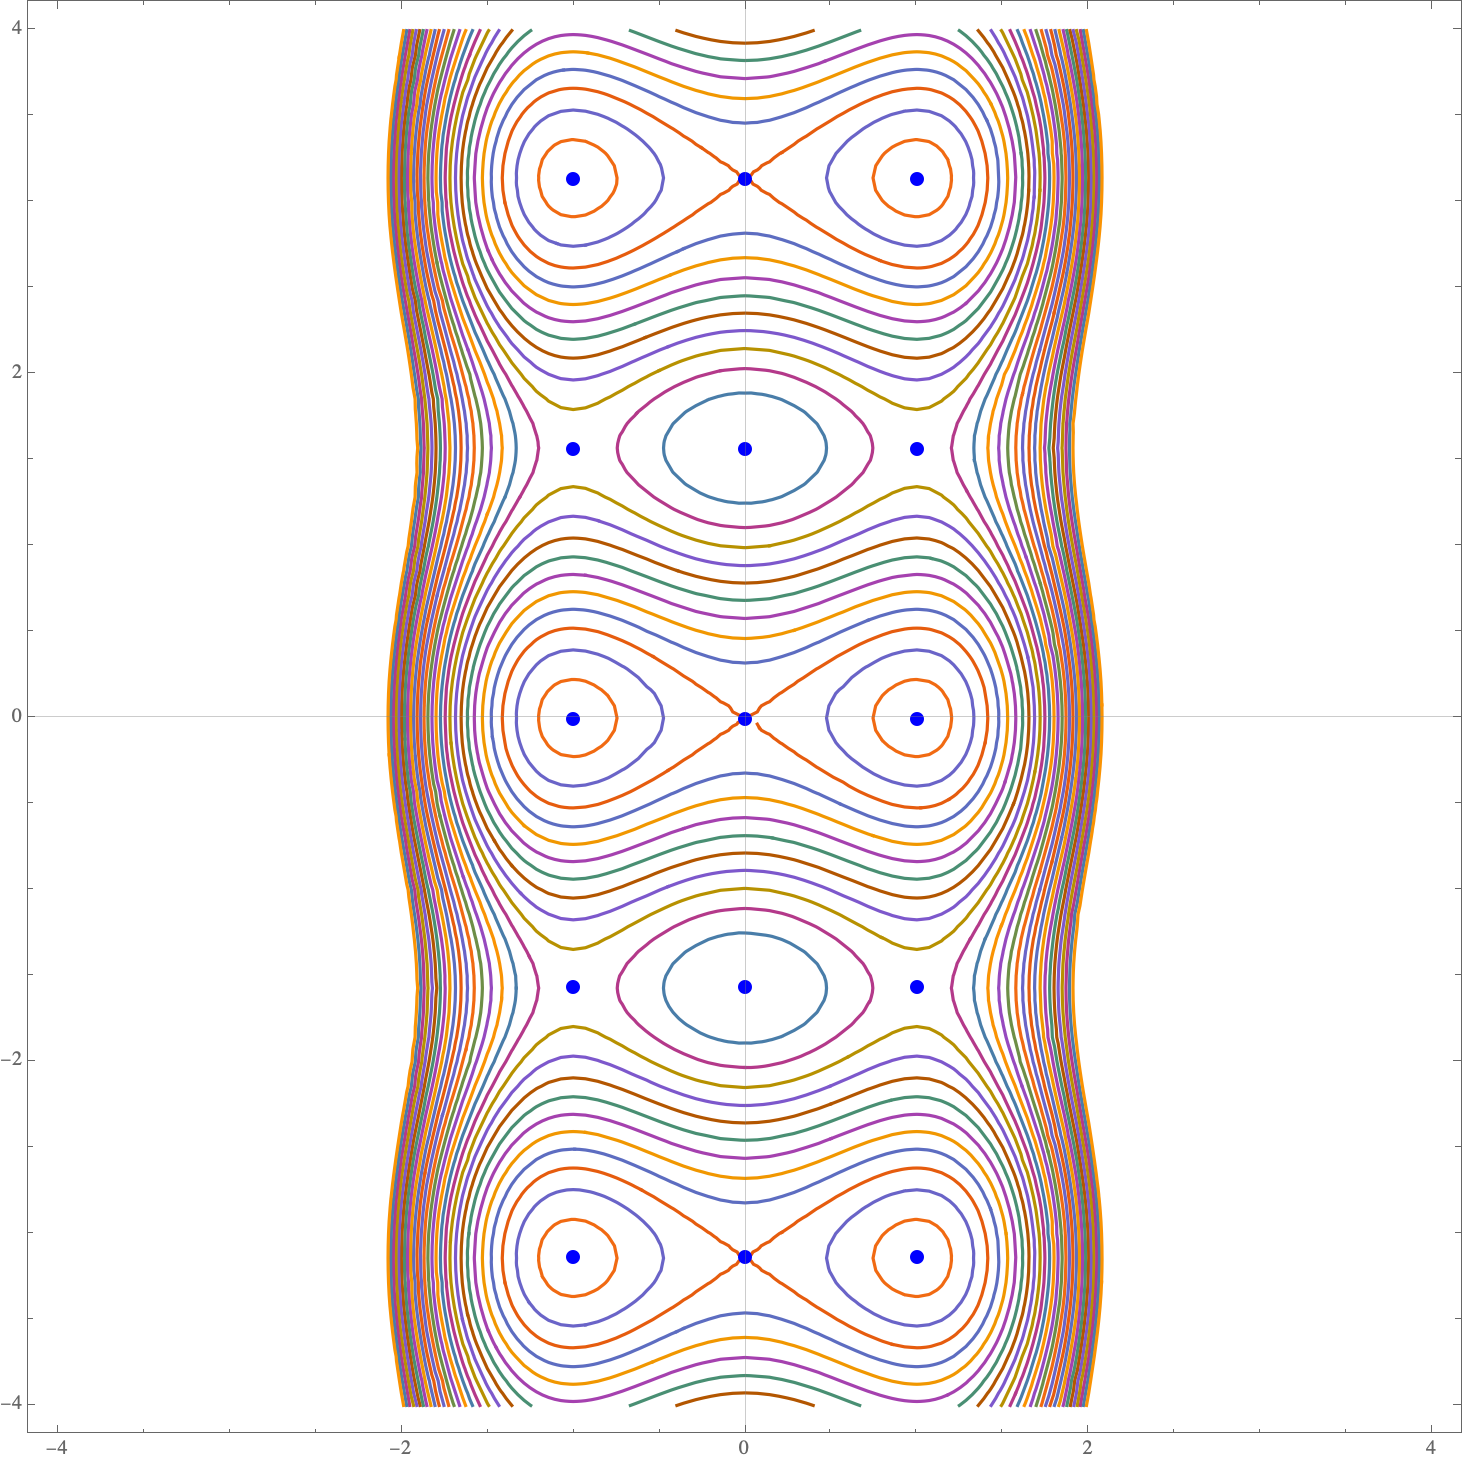
\includegraphics[width=0.7\textwidth]{images/test_3/diff_eq.png}
    \caption{Сімейство кривих $\frac{x^4}{4}-\frac{x^2}{2}+\frac{\cos 2y}{2}=C$ для $C \in [-2,2]$}
    \label{fig:1}
\end{figure}

Добре видно, що точки, що ми до цього знайшли (а саме $\begin{bmatrix}
    0 \\ \frac{\pi(2m+1)}{2}
\end{bmatrix}$ та $\begin{bmatrix}
    \pm 1 \\ \pi m
\end{bmatrix}$ для $m \in \mathbb{Z}$) дійсно виглядають, як седла. А ось точки, характер яких ми не могли визначити, дуже схожі на ``центри'', оскільки маємо сімейство замкнутих кривих навколо них. 

\textbf{Відповідь.}

\begin{enumerate}
    \item $\begin{bmatrix}
    0 \\ \frac{\pi(2m+1)}{2}
\end{bmatrix}$ та $\begin{bmatrix}
    \pm 1 \\ \pi m
\end{bmatrix}$ для $m \in \mathbb{Z}$ є седлами.
\item $\begin{bmatrix}
    0 \\ \pi m
\end{bmatrix}$ та $\begin{bmatrix}
    \pm 1 \\ \frac{\pi(2m+1)}{2}
\end{bmatrix}$ для $m \in \mathbb{Z}$ є центрами.
\end{enumerate}

\pagebreak
\section*{Завдання 3.}

\textbf{Умова.} Дослідити нульовий розв'язок на стійкість методом Ляпунова
\[
\begin{cases}
    \dot{x} = 2y^5 - x^5 \\
    \dot{y} = -x-3y^3
\end{cases}
\]

\textbf{Розв'язок.} Одразу будемо шукати функцію Ляпунова у наступному вигляді:
\[
V(x,y) = \alpha x^{2n} + \beta y^{2m}, \; \alpha,\beta>0
\]
Тоді:
\begin{gather*}
\dot{V}(x,y) = 2\alpha n x^{2n-1}\dot{x} + 2\beta m y^{2m-1} \dot{y} \\
= 2\alpha n x^{2n-1}(2y^5 - x^5) + 2\beta m y^{2m-1}(-x-3y^3) \\
= -2\alpha n x^{2n+4} + 4\alpha n x^{2n-1}y^5 - 2\beta m y^{2m-1}x - 6\beta m y^{2m+2}
\end{gather*}
Нам бажано позбавитись знакозмінного виразу $4\alpha n x^{2n-1}y^5 - 2\beta m y^{2m-1}x$. Отже, маємо вимагати в такому випадку
\[
4\alpha n x^{2n-1}y^5 = 2\beta m y^{2m-1}x
\]
Спочатку прирівнюємо ступені. Маємо $2n-1=1 \implies n=1$, а також $2m-1=5 \implies m=3$. Тепер прирівнюємо коефіцієнти, маємо:
\[
4\alpha n = 2\beta m \implies 4\alpha = 6\beta \implies 2\alpha = 3\beta
\]
Для зручності покладемо $\alpha=3,\beta=2$. Остаточно, отримали наступну функцію Ляпунова:
\[
V(x,y) = 3x^2 + 2y^6,
\]
похідна якої:
\[
\dot{V}(x,y) = -6x^6 - 36y^8
\]
Бачимо, що виконуються $\forall (x,y) \in \mathbb{R}^2 \setminus \{(0,0)\}: \dot{V}(x,y) < 0$, а отже розв'язок є \textbf{стійким}.

\textbf{Відповідь.} Функція Ляпунова $V(x,y)=3x^2+2y^6$, нульовий розв'язок \textbf{стійкий}.

\end{document}

